% ScriptConsist: Threws Odyssey 2026, Applied Research
% Compile with XeLaTeX (Devanagari):  latexmk -xelatex main.tex
\documentclass[11pt]{article}
\usepackage[preprint]{acl}

\usepackage{fontspec}
\setmainfont{texgyretermes}[Extension=.otf, UprightFont=*-regular, BoldFont=*-bold,
  ItalicFont=*-italic, BoldItalicFont=*-bolditalic]
\newfontfamily\devfont[Script=Devanagari, Scale=0.93]{FreeSerif}
\newcommand{\hi}[1]{{\devfont #1}}

\usepackage{microtype}
\usepackage{graphicx}
\usepackage{booktabs}
\usepackage{multirow}
\usepackage{amsmath}
\usepackage{xcolor}
\usepackage{tabularx}

\newcommand{\pp}{\,pp}
\newcommand{\Dev}{Devanagari}
\newcommand{\Rom}{rule-based Roman}
\newcommand{\Hng}{natural Hinglish}
\newcommand{\HngC}{Natural Hinglish}
\newcommand{\RomC}{Rule-based Roman}

\title{ScriptConsist: Separating Script from Natural Code-Mixing\\in LLM Factual Recall for Hindi}

\author{Aadeesh Surana \\
  Indian Institute of Information Technology Vadodara \\
  \texttt{aadeeshsurana01@gmail.com}}

\begin{document}
\maketitle

\begin{abstract}
Hindi speakers type questions to language models in at least three ways: in English, in Devanagari, and in Roman script mixed with English words (Hinglish).
Benchmarks for Hindi almost always use Devanagari, and studies of romanized input usually generate it automatically.
We introduce \textbf{ScriptConsist}, 296 factual questions from Mintaka and IndicQuest, each in four parallel forms: English, \Dev{} Hindi, a rule-based romanization of that \Dev{} (same words, Roman script), and Hinglish typed by a native speaker.
Comparing \Dev{} with its rule-based romanization isolates the effect of \emph{script}; comparing the rule-based and typed versions isolates \emph{natural typing}.
We evaluate seven open 4--9B models, three of them Hindi-focused, with three prompt wordings per form (33{,}939 answers), using a cross-script answer matcher that agrees with blind human judgments at Cohen's $\kappa = 0.95$.
Every model is more accurate on \Hng{} than on \Dev{}, by 10--33 points, and \Hng{} comes within 3--15 points of English.
Rule-based romanization is the least accurate form for every model, but the cost of changing script alone ranges from 1 to 42 points.
These results hold after correcting for scorer error and across quantization and prompt wording.
Evaluating Hindi only in \Dev{}, or with synthetic transliteration, misstates how well models answer the questions Hindi speakers actually type.
\end{abstract}

% =====================================================================
\section{Introduction}

A Hindi speaker who wants to know when George Orwell died might type \emph{When did George Orwell die?}, \hi{जॉर्ज ऑरवेल की मृत्यु कब हुई थी}?, or \emph{George Orwell kab mare the?}
The third form, Hindi in Roman script with English words mixed in, is how a large share of everyday Hindi is typed on phones.
Yet multilingual factual-knowledge benchmarks for Hindi are written in Devanagari \citep{rohera2024indicquest,jain2026indicquestv2}, and studies that do test Roman script mostly generate it by transliteration \citep{das2026indiromcom}.

Two things change at once when a question moves from Devanagari to natural Hinglish: the \emph{script} (Devanagari to Latin) and the \emph{wording} (Hindi words replaced by English ones, names spelled the English way, informal spelling).
Earlier comparisons cannot tell these apart, so it is unclear whether a model's weakness in ``Hindi'' comes from the language, the script, or the way people actually type.

We build a benchmark that separates them.
Each ScriptConsist question has four parallel forms (Table~\ref{tab:examples}).
The rule-based romanization uses exactly the words of the Devanagari question, so \Dev{} vs.\ \Rom{} differs only in script.
The \Hng{} was typed by a native speaker without a scheme, so \Rom{} vs.\ \Hng{} differs only in wording, within the same script.

\begin{table}[t]
\centering\small
\begin{tabularx}{\columnwidth}{@{}lX@{}}
\toprule
English & When did George Orwell die? \\
\Dev{} & \hi{जॉर्ज ऑरवेल की मृत्यु कब हुई थी}? \\
\RomC{} & Jorj orvel ki mrityu kab hui thi? \\
\HngC{} & George Orwell kab mare the? \\
\midrule
English & Which city is known as the Manchester of India? \\
\Dev{} & \hi{किस शहर को भारत का मैनचेस्टर कहा जाता है}? \\
\RomC{} & Kis shahar ko bharat ka mainachestar kaha jata hai? \\
\HngC{} & Kaunsi city ko Manchester of India kehte hain? \\
\bottomrule
\end{tabularx}
\caption{Two ScriptConsist items in their four forms (gold answers: 1950; Ahmedabad). The rule-based form keeps the Devanagari wording and changes only the script; the natural Hinglish was typed by a native speaker.}
\label{tab:examples}
\end{table}

\paragraph{Contributions.}
\begin{itemize}\setlength\itemsep{0pt}
\item \textbf{ScriptConsist}, 296 factual short-answer questions in four parallel forms, built from Mintaka \citep{sen2022mintaka} and IndicQuest \citep{rohera2024indicquest}. Every gold answer was checked, and every keep/drop decision is logged with a reason.
\item \textbf{A design that decomposes the Hindi gap} into a script effect and a natural-typing effect.
\item \textbf{An evaluation of seven open models} (Qwen2.5-7B, Llama-3.1-8B, Aya-Expanse-8B, Gemma-2-9B, and the Hindi-focused Nemotron-4-Mini-Hindi-4B, Airavata and Gajendra), plus 4-bit versions of two of them, with a cross-script scorer validated against blind human judgments.
\item \textbf{Findings.} \HngC{} beats \Dev{} for every model, and synthetic romanization is the worst form. A benchmark that uses \Dev{} or transliteration alone therefore underestimates what models know when asked the way users type.
\end{itemize}

% =====================================================================
\section{Related Work}

\paragraph{Cross-lingual factual consistency.}
\citet{qi2023crosslingual} showed that multilingual models often give different factual answers to the same question in different languages.
For Indian languages, IndicQuest \citep{rohera2024indicquest} provides 200 India-focused questions in English and 19 Indic languages, and models answer them better in English, even for questions about India \citep{rohera2025better}.
IndicQuest~v2 \citep{jain2026indicquestv2} scales this to 3{,}471 questions.
All of these use native script only.

\paragraph{Romanized and code-mixed input.}
RomanSetu \citep{husain2024romansetu} found that representing Indic text in Roman script can help English-centric models, after continued pretraining on romanized data.
In a real-world medical triage setting, \citet{khullar2025scriptgap} found models perform worse on romanized messages than on native-script ones, with gaps of up to 24 points.
Indi-RomCoM \citep{das2026indiromcom} tests synthetic code-mixed, romanized instructions at controlled mixing levels, without a native-script condition.
IndoTranslit \citep{gharami2025indotranslit} targets transliteration of noisy romanized Hindi and Bengali.
To our knowledge, no benchmark compares the same factual questions in native script, rule-based romanization and \emph{naturally typed} Hinglish, which is what separates script from typing.

\paragraph{Hindi-focused models.}
Airavata \citep{gala2024airavata} and Gajendra \citep{bhabha2024gajendra} are instruction-tuned models built on OpenHathi, a Llama-2 extension for Hindi. Gajendra was also trained on Hinglish.
Nemotron-4-Mini-Hindi-4B \citep{joshi2024nemotronhindi} was adapted to Hindi through continued pretraining with synthetic data.

% =====================================================================
\section{The ScriptConsist Benchmark}

\subsection{Sources and filtering}

\paragraph{Mintaka.}
Mintaka \citep{sen2022mintaka} has 18{,}000 English questions (we merge train and test), with professional Hindi translations and answers linked to Wikidata.
We keep five question types (generic, superlative, intersection, multi-hop, ordinal) whose answer is an entity with a Hindi Wikidata label, or a date scored on the year.
We drop yes/no and comparative questions (guessable), count and difference questions (answers drift), and questions that are time-sensitive, list their answer options, leak the answer, contain Latin script inside the Hindi, rely on an implicit US context (``What state grows potatoes?'' reads as an Indian state in Hindi), or ask about records that can change after 2022 (``best-selling'', ``of all time'').
Of 18{,}000 questions, 3{,}685 pass.
We draw a seeded sample of 300, stratified over Mintaka's eight topics and question types.

\paragraph{IndicQuest.}
We reviewed all 200 English--Hindi pairs of IndicQuest \citep{rohera2024indicquest} by hand and kept 81. The 119 drops were mostly descriptive or essay questions (59); the rest had multiple valid answers, were ambiguous, multi-part, time-sensitive, or had a wrong gold answer.
We extracted a short gold answer from each sentence answer.

\paragraph{Answer checks and rejections.}
The author checked every gold answer, mostly against cited sources.
For Mintaka, the author corrected 4 gold answers and rejected 16 items as ambiguous or unverifiable.
A second review rejected 39 more: ambiguity, two valid answers, records that changed after 2022, and one Hinglish question that changed the meaning.
It also removed 7 near-duplicates, corrected 2 gold answers and extended 3 answer-variant lists.
Of the 81 IndicQuest items, 61 were annotated within the project's time and 3 were rejected.
The frozen benchmark has \textbf{296 items}: 238 from Mintaka and 58 from IndicQuest.
Every rejection is listed with its reason in the released files.

\subsection{The four forms}
\begin{description}\setlength\itemsep{0pt}
\item[English] the source question.
\item[\Dev{}] Mintaka's professional translation, or IndicQuest's released Hindi (machine-translated), both unedited.
\item[\RomC{}] a deterministic transliteration of the \Dev{}: Aksharamukha IAST \citep{rajan2026aksharamukha} with Hindi schwa deletion, reduced to ASCII (\hi{मृत्यु} $\to$ \emph{mrityu}).
\item[\HngC{}] typed on a phone by the author, a native Hindi speaker, as if messaging a friend, with no transliteration scheme and English words used freely. On average 44\% of its words come from the English question.
\end{description}
A second native speaker had earlier typed 73 of the questions.
The author retyped all of them, so every evaluated \Hng{} question has a single typist.
The second speaker's versions are kept as a fifth form for those 73 items, to measure sensitivity to the typist.
The two versions matched exactly in only 5 of 73 cases (7\%); mean character similarity was 0.85.
Eight Hinglish questions that changed the meaning of the original were retyped after review; a ninth was rejected.

\subsection{Composition}
Answers are entities (223), years (67) or numbers (6).
The items cover History (52), Geography (46), Politics (44), Books, Movies and Music (30 each), Sports (27), Video Games (26), Economics (7) and Literature (4).
53 questions are about India; all of them come from IndicQuest.
The other 243 are about global topics, almost all from Mintaka.
Locality and source are therefore confounded, which we keep in mind in \S\ref{sec:locality}.

% =====================================================================
\section{Experimental Setup}

\paragraph{Models.}
We evaluate Qwen2.5-7B-Instruct \citep{qwen2024qwen25}, Llama-3.1-8B-Instruct \citep{grattafiori2024llama3}, Aya-Expanse-8B \citep{dang2024aya}, Nemotron-4-Mini-Hindi-4B-Instruct \citep{joshi2024nemotronhindi}, Airavata \citep{gala2024airavata} and Gajendra-v0.1 \citep{bhabha2024gajendra} in float16.
Gemma-2-9B-it \citep{gemma2024gemma2} is unstable in float16 and the T4 GPUs we used lack bfloat16, so it runs in 4-bit NF4 \citep{dettmers2023qlora} with float32 compute.
To measure the effect of quantization, Qwen and Llama also run in NF4, since 4-bit quantization is known to hurt non-Latin scripts more \citep{marchisio2024quantization}.
Each model uses its own chat format (Tulu for Airavata, ChatML for Gajendra).

\paragraph{Prompts and decoding.}
Each question is asked with three instruction wordings (e.g.\ ``Answer the following question with only the answer\ldots'').
The instruction is written in the same form as the question, so no other script leaks into the prompt; the \Rom{} instructions are themselves rule-based transliterations of the Devanagari ones.
Decoding is greedy with at most 48 new tokens.
Each run has 3{,}771 prompts: 296 items $\times$ 4 forms $\times$ 3 wordings, plus the 73 second-typist questions.
Nine runs give 33{,}939 answers.
All runs used free Kaggle notebooks (2$\times$ NVIDIA T4).

\paragraph{Scoring.}
A model asked in Hindi may answer \hi{मार्क ट्वैन}, \emph{Mark Twain}, or a full sentence.
The matcher accepts an answer in any script.
Years match on any 3--4 digit number, with Devanagari digits converted.
For entities, the matcher looks for a gold variant (English, Devanagari, or its romanization) as whole words, then on a romanized copy of the answer.
Failing that, it requires every distinctive word of the gold name, compared on spelling and on a consonant skeleton so that \hi{मेडिसन} and \hi{मैडिसन} match, with a guard that numbers must agree.
Every decision records which rule fired.
68 unit tests cover the failure cases found while auditing the scorer.
The scorer was then frozen and validated (\S\ref{sec:validation}).

\paragraph{Statistics.}
Per question, accuracy is the mean over the three wordings.
Confidence intervals are 95\% bootstrap intervals over questions (10{,}000 resamples).
Paired differences are tested with a sign-flip permutation test over questions, and $p$-values are Holm-corrected \citep{holm1979} within each family of tests (35 tests for the gaps in Figure~\ref{fig:gaps}).

% =====================================================================
\section{Scorer Validation}
\label{sec:validation}

Automatic matching across scripts can fail in exactly the conditions we compare, for example by missing correct Devanagari spellings of foreign names.
We therefore validated the frozen scorer on a blind sample of answers.
For each of the four forms we drew 75 answers from the five general models, half accepted and half rejected by the scorer, plus 10 from Airavata and Gajendra.
The author judged each one in a web form showing the question, the gold answer and the model's answer, without the scorer's verdict or the model's name.
To check the validator's own consistency, 48 answers were shown a second time under new ids, at least 90 positions later.

\begin{table}[t]
\centering\small
\begin{tabular}{@{}lrccc@{}}
\toprule
Form & $n$ & $\kappa$ & False acc. & Missed \\
\midrule
English & 83 & 0.93 & 0/43 & 3/40 \\
\Dev{} & 83 & 0.95 & 0/43 & 2/40 \\
\RomC{} & 83 & 0.98 & 1/43 & 0/40 \\
\HngC{} & 82 & 0.95 & 0/42 & 2/40 \\
\midrule
All & 331 & 0.95 & 1/171 & 7/160 \\
\bottomrule
\end{tabular}
\caption{Scorer vs.\ blind human judgment. False acc.: scorer accepted, human rejected. Missed: scorer rejected, human accepted. Nine answers judged ``unsure'' are excluded; counting them as wrong gives $\kappa = 0.95$ overall.}
\label{tab:validation}
\end{table}

Table~\ref{tab:validation} shows the result.
Agreement is 97.6\% ($\kappa = 0.95$; \citealp{cohen1960kappa}), and at least 0.93 in every form.
The scorer accepted one wrong answer, a year range (``1517--1519'') counted as the gold 1519.
It missed seven correct ones.
Two of these were paraphrases (``self-inflicted gunshot wound'' for \emph{suicide}) or acronyms (\emph{LDP}).
Most of the rest were lenient human calls, such as accepting \emph{The Lord of the Rings} for \emph{The Fellowship of the Ring}.
On the 40 answers from the two Hindi-focused models, agreement was perfect.
The validator gave the same verdict to 47 of the 48 repeated answers; the one change was from ``wrong'' to ``unsure''.

\paragraph{Correcting for scorer error.}
Because the sample is stratified on the scorer's verdict, it estimates, for each form, the false-accept rate $\mathrm{FA}$ and the missed-correct rate $M$.
The corrected accuracy of a run is $a(1-\mathrm{FA}) + (1-a)M$.
Correction changes accuracies by at most 5.1 points and changes no ordering of forms or models.
We then propagated the uncertainty in each form's error rates by drawing them from Beta posteriors 20{,}000 times.
In every run, \Hng{} stays above \Dev{} with probability at least 0.99.
\Dev{} stays above \Rom{} with probability above 0.98 for six runs, but only 0.97 and 0.96 for Qwen (float16, 4-bit) and 0.93 for Gajendra, whose uncorrected gaps are already small (\S\ref{sec:decomp}).

% =====================================================================
\section{Results}

\begin{figure}[t]
\centering
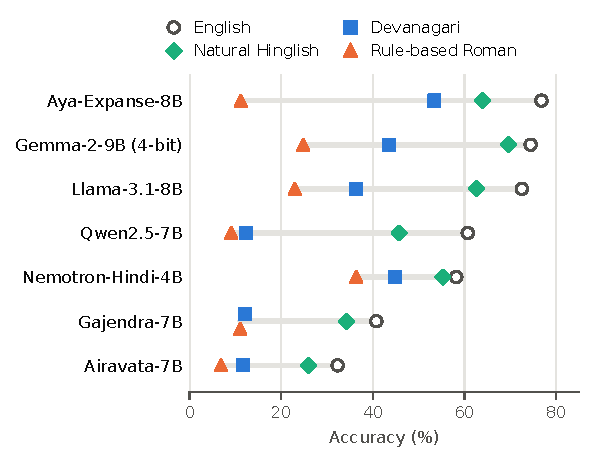
\includegraphics[width=\columnwidth]{figures/fig_accuracy.pdf}
\caption{Accuracy by question form. Every model is more accurate on \Hng{} than on \Dev{}, and least accurate on the \Rom{} form. 95\% CIs are in Table~\ref{tab:acc}.}
\label{fig:acc}
\end{figure}

\begin{table*}[t]
\centering\small\setlength\tabcolsep{4.5pt}
\begin{tabular}{@{}lccccc@{}}
\toprule
Model & English & \Dev{} & \RomC{} & \HngC{} & Hinglish, 2nd typist ($n$=73) \\
\midrule
Qwen2.5-7B & 60.7 {\scriptsize[55.5, 65.8]} & 12.4 {\scriptsize[9.2, 15.8]} & 9.1 {\scriptsize[6.6, 11.7]} & 45.7 {\scriptsize[40.9, 50.6]} & 44.3 {\scriptsize[34.2, 54.8]} \\
Llama-3.1-8B & 72.5 {\scriptsize[67.9, 76.9]} & 36.4 {\scriptsize[31.4, 41.3]} & 23.0 {\scriptsize[18.9, 27.3]} & 62.6 {\scriptsize[57.6, 67.5]} & 53.4 {\scriptsize[43.4, 63.9]} \\
Aya-Expanse-8B & \textbf{76.8} {\scriptsize[72.2, 81.3]} & \textbf{53.4} {\scriptsize[48.3, 58.5]} & 11.2 {\scriptsize[8.7, 13.9]} & 64.0 {\scriptsize[59.2, 68.6]} & 53.9 {\scriptsize[43.8, 63.9]} \\
Gemma-2-9B (4-bit) & 74.4 {\scriptsize[69.7, 79.2]} & 43.5 {\scriptsize[38.2, 48.9]} & 24.8 {\scriptsize[20.6, 29.4]} & \textbf{69.6} {\scriptsize[64.6, 74.3]} & 61.6 {\scriptsize[51.1, 71.7]} \\
Nemotron-Hindi-4B & 58.2 {\scriptsize[53.4, 63.2]} & 44.8 {\scriptsize[39.9, 50.0]} & \textbf{36.4} {\scriptsize[31.6, 41.0]} & 55.3 {\scriptsize[50.2, 60.4]} & 49.3 {\scriptsize[39.7, 58.9]} \\
Airavata-7B & 32.3 {\scriptsize[27.4, 37.3]} & 11.7 {\scriptsize[8.7, 15.1]} & 6.9 {\scriptsize[4.8, 9.1]} & 25.9 {\scriptsize[21.6, 30.4]} & 26.0 {\scriptsize[17.3, 35.2]} \\
Gajendra-7B & 40.8 {\scriptsize[35.8, 45.8]} & 12.0 {\scriptsize[9.1, 15.2]} & 11.0 {\scriptsize[8.5, 14.0]} & 34.2 {\scriptsize[29.6, 39.0]} & 33.3 {\scriptsize[24.2, 42.9]} \\
\midrule
Qwen2.5-7B (4-bit) & 56.8 {\scriptsize[51.5, 61.8]} & 10.9 {\scriptsize[7.9, 14.2]} & 8.1 {\scriptsize[5.7, 10.7]} & 43.2 {\scriptsize[38.3, 48.1]} & 45.2 {\scriptsize[35.2, 55.2]} \\
Llama-3.1-8B (4-bit) & 70.2 {\scriptsize[65.4, 74.8]} & 29.9 {\scriptsize[25.3, 34.7]} & 21.3 {\scriptsize[17.3, 25.4]} & 59.2 {\scriptsize[54.3, 64.1]} & 52.5 {\scriptsize[42.5, 63.0]} \\
\bottomrule
\end{tabular}
\caption{Accuracy (\%) on the 296 questions, averaged over three prompt wordings, with 95\% bootstrap CIs over questions. Best per column in bold (top block). The last column covers the 73 questions also typed by a second speaker.}
\label{tab:acc}
\end{table*}

\subsection{Natural Hinglish beats Devanagari}
Figure~\ref{fig:acc} and Table~\ref{tab:acc} give accuracy by form.
English is the most accurate form for every model, and \Hng{} is second for every model.
Its distance from English is 3--15 points: 2.9 for Nemotron-Hindi (not significant), 4.8 for Gemma, and 15.0 for Qwen.
\Dev{} is far behind: \Hng{} beats it by 10.5 (Nemotron) to 33.3 points (Qwen), significant for all seven models (Figure~\ref{fig:gaps}c).
Even Aya-Expanse, the best model in \Dev{} at 53.4\%, does 10.6 points better in \Hng{}.

The Hindi-focused models do not reverse this.
Nemotron-Hindi has the smallest gaps between forms.
Airavata is the least accurate model in every form, and its \Dev{} accuracy (11.7\%) and Gajendra's (12.0\%) are no higher than Qwen's (12.4\%).

\begin{figure*}[t]
\centering
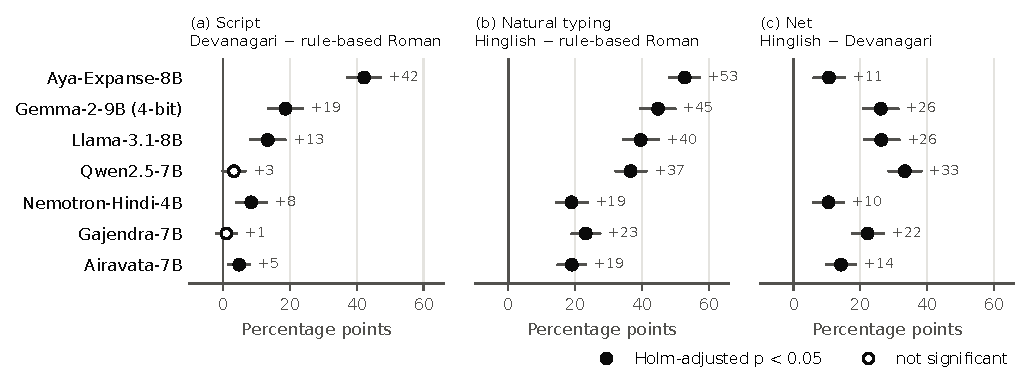
\includegraphics[width=\textwidth]{figures/fig_gaps.pdf}
\caption{Paired accuracy differences with 95\% bootstrap CIs (percentage points). (a) Same words, different script. (b) Same script, natural vs.\ rule-based wording. (c) The net difference between the two Hindi forms users actually type. Filled: Holm-adjusted $p<0.05$ over 35 tests.}
\label{fig:gaps}
\end{figure*}

\subsection{Script vs.\ natural typing}
\label{sec:decomp}
Figure~\ref{fig:gaps} splits the difference.

\paragraph{Script (a).}
Writing the same Hindi words in Roman script always lowers accuracy, but by very different amounts.
The drop is 42.2 points for Aya and 13--19 for Llama and Gemma.
It is 3.3 for Qwen and 1.0 for Gajendra, neither significant; both models are already near the floor in \Dev{}.
A strict transliteration is thus an unfamiliar input for most models, not a neutral re-encoding.
Notably, when asked in \Rom{}, Aya answers in Devanagari 78\% of the time (Llama: never), which suggests it recognizes the language but not the spelling convention.

\paragraph{Natural typing (b).}
Within Roman script, replacing the rule-based version with the typed Hinglish raises accuracy by 19 points (Nemotron, Airavata) to 53 points (Aya), significant for every model.
This is the largest effect in the study.
It is not explained by how much English the Hinglish contains: the share of English words per question has no significant correlation with the gain for any model (Spearman $|\rho| \le 0.09$).
The typed Hinglish usually keeps names in their English spelling (\emph{George Orwell}, not \emph{Jorj orvel}).
In 82\% of the questions that contain names, it keeps every one, which leaves too little variation to test this explanation.
The gain is larger when all names are kept for six of seven models, but no correlation is significant after correction.

\paragraph{Net (c).}
\HngC{} beats \Dev{} for every model.
For most models the natural-typing gain in (b) is far larger than the script cost in (a), so the form users actually type does better than the native-script form benchmarks use.

\subsection{India-specific questions}
\label{sec:locality}

\begin{figure*}[t]
\centering
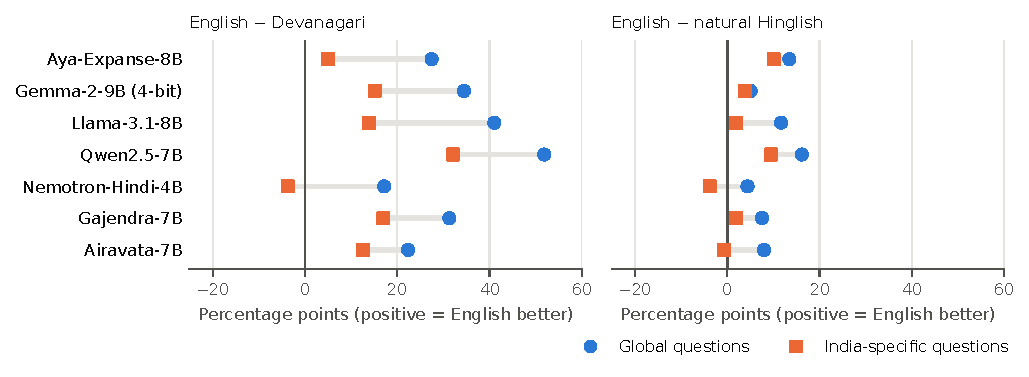
\includegraphics[width=\textwidth]{figures/fig_locality.pdf}
\caption{English advantage on India-specific ($n=53$, all from IndicQuest) vs.\ global questions ($n=243$, almost all from Mintaka). The advantage shrinks on India-specific questions for every model, but locality is confounded with source and with Devanagari translation quality (machine translation for IndicQuest), so this comparison is descriptive.}
\label{fig:locality}
\end{figure*}

The English advantage over both Hindi forms is smaller on the 53 India-specific questions for all seven models (Figure~\ref{fig:locality}).
Nemotron-Hindi is 3.8 points \emph{more} accurate in \Dev{} and in \Hng{} than in English on these questions.
Because every India-specific question comes from IndicQuest, whose Hindi is machine-translated, we report this as descriptive.

\subsection{Robustness}

\paragraph{Quantization.}
NF4 lowers accuracy by up to 6.4 points; the significant drops are Qwen in English ($-3.9$) and Llama in \Dev{} ($-6.4$).
NF4 does not significantly widen the gap between English and either Hindi form for either model (difference-in-differences, Holm-corrected), and the ordering of forms is identical at both precisions (Table~\ref{tab:acc}).

\paragraph{Typist.}
On the 73 questions typed by both speakers, average accuracy does not differ significantly between the two versions for six of seven models.
The exception is Airavata, which does 11.0 points better on the author's version.
Individual questions still flip: per question, accuracy differs by 6--13 points on average between the two typists' versions.
The aggregate result is thus stable, but single-item results depend on spelling.

\paragraph{Prompt wording.}
Across the three instruction wordings, accuracy varies by at most 6.8 points per model in each of the four main forms.
The exception is Aya on \Rom{} (12.8 points), consistent with that input being unfamiliar.

\subsection{Answer behaviour}
The scorer accepts answers in any script, but the script models choose is informative.
Asked in \Dev{}, models answer in Devanagari 72--93\% of the time.
Asked in \Hng{}, they rarely answer in Devanagari (under 2\%), except Aya (28\%).
Qwen sometimes switches to Chinese or Japanese characters: 5.1\% of its answers to \Dev{} questions.
Airavata and Gajendra sometimes answer with a placeholder instead of a name, such as \hi{नाम} \_ 1 (1--5\% of answers per form).
This suggests anonymized names in their training data, though we cannot verify the source.

% =====================================================================
\section{Discussion}

\paragraph{What the decomposition shows.}
If the Hindi gap were about the language, \Hng{} and \Dev{} would perform alike.
If it were about the script, \Rom{} would perform like \Hng{}.
Neither is the case.
Script matters, sometimes a great deal, but the larger factor is whether the input looks like text the model has seen.
Natural Hinglish, with English spellings of names and common English words, sits much closer to that text than either a formal Devanagari translation or a strict transliteration.
We could not isolate which feature of natural typing matters most.
Name spelling is the most plausible candidate, but our data has too little variation to test it.

\paragraph{Implications for evaluation.}
A Devanagari-only benchmark underestimates what models know when Hindi speakers ask the way they type: by 10--33 points on our questions.
A synthetic-romanization benchmark underestimates it even more.
Conversely, a model's English score overstates what Devanagari users get by 13--48 points.
Benchmarks for languages that are commonly romanized should include at least one naturally typed form.

\paragraph{For model builders.}
The two models fine-tuned for Hindi on a Llama-2 base were among the weakest, including in Devanagari: Airavata was last in every form.
The Hindi-adapted Nemotron model had the most even profile across forms but not the highest accuracy.
Adaptation alone does not close the gap; a stronger base model matters more on these questions.

% =====================================================================
\section{Limitations}

\begin{itemize}\setlength\itemsep{0pt}
\item \textbf{One typist.} All evaluated \Hng{} was typed by one person, the author. A second speaker's versions of 73 questions agree with ours in aggregate, but other people type differently. The two versions matched word for word only 7\% of the time.
\item \textbf{One validator, who is also the author.} Blinding and the repeated-item check reduce, but do not remove, this concern. A second independent rater would strengthen the validation.
\item \textbf{Translation quality.} The Devanagari is unedited: professional for Mintaka (it contains some spelling errors) and machine-translated for IndicQuest. Better Devanagari might narrow the gap to \Hng{}.
\item \textbf{Scope.} The study covers 296 questions, mostly about global topics, with only 53 about India. It tests open 4--9B models only, with greedy decoding. Larger and closed models may behave differently.
\item \textbf{Prompt confound.} The \Hng{} and \Rom{} prompts differ in their instruction wording as well as in the question. Three wordings per form limit, but do not remove, this effect.
\end{itemize}

\section*{Ethics and Licensing}
ScriptConsist derives from Mintaka (CC BY 4.0) and IndicQuest (CC BY-NC-SA 4.0), and is released under CC BY-NC-SA 4.0.
The questions concern public facts and contain no personal data about private individuals.
The annotation work was done by the author.
All code, data, model outputs, human judgments and the decision logs are released.

\section*{Acknowledgments}
We thank the second native speaker who typed an earlier version of 73 questions, which made the typist comparison possible.

\bibliography{references}

\end{document}
